% https://www.overleaf.com/learn/latex/Beamer#Using_a_colorthemev

% Inbuilt themes in beamer
\documentclass[8pt, aspectratio=169]{beamer}

\input{../template/macros/macros_general.tex}
\input{../template/macros/macros_math.tex}
\input{../template/symbols/symbols_NN.tex}
\input{../template/symbols/symbols_robot.tex}

% % Theme choice:
% \usetheme{Antibes}
% % \usecolortheme{beaver}
%~~~~~~~~~~~~~~~~~~~~~~~~~~~~~~~~~~~~~~~~~~~~~~~~~~~~~~~~~~~~~~~~~~~~~~~~~~~~~~
% Use roboto Font (recommended)
\usepackage[sfdefault]{roboto}
\usepackage[utf8]{inputenc}
\usepackage[T1]{fontenc}
%~~~~~~~~~~~~~~~~~~~~~~~~~~~~~~~~~~~~~~~~~~~~~~~~~~~~~~~~~~~~~~~~~~~~~~~~~~~~~~

%~~~~~~~~~~~~~~~~~~~~~~~~~~~~~~~~~~~~~~~~~~~~~~~~~~~~~~~~~~~~~~~~~~~~~~~~~~~~~~
% Use roboto Font (recommended)
\usepackage[sfdefault]{roboto}
\usepackage[utf8]{inputenc}
\usepackage[T1]{fontenc}
%~~~~~~~~~~~~~~~~~~~~~~~~~~~~~~~~~~~~~~~~~~~~~~~~~~~~~~~~~~~~~~~~~~~~~~~~~~~~~~

%~~~~~~~~~~~~~~~~~~~~~~~~~~~~~~~~~~~~~~~~~~~~~~~~~~~~~~~~~~~~~~~~~~~~~~~~~~~~~~
% Define where theme files are located. ('/styles')
\usepackage{styles/fluxmacros}
\usefolder{styles}
% Use Flux theme v0.1 beta
% Available style: asphalt, blue, red, green, gray 
\usetheme[style=blue]{flux}
%~~~~~~~~~~~~~~~~~~~~~~~~~~~~~~~~~~~~~~~~~~~~~~~~~~~~~~~~~~~~~~~~~~~~~~~~~~~~~~

%~~~~~~~~~~~~~~~~~~~~~~~~~~~~~~~~~~~~~~~~~~~~~~~~~~~~~~~~~~~~~~~~~~~~~~~~~~~~~~
% Extra packages for the demo:
\usepackage{booktabs}
\usepackage{colortbl}
\usepackage{ragged2e}
\usepackage{schemabloc}
%~~~~~~~~~~~~~~~~~~~~~~~~~~~~~~~~~~~~~~~~~~~~~~~~~~~~~~~~~~~~~~~~~~~~~~~~~~~~~~
\usepackage{calc}

% Title page details: 
\title{
    Imposing a Weight Norm Constraint for Neuro–Adaptive Control 
} 
\subtitle{
    \textit{IEEE European Control Conference (ECC) 2025}\\
}
\author{Myeongseok Ryu\inst{1}, Jiyun Kim\inst{2}, and Kyunghwan Choi\inst{1}}
\date{\today}
% \institute[short]{\inst{1} First \samelineand \inst{2} Second \samelineand \inst{3} Third}
\newcommand{\samelineand}{\\}
\institute{%
    \begin{minipage}[c]{\linewidth}
        \centering
        \inst{1}%
        Department of Mechanical and Robotics Engineering\\
        Gwangju Institute of Science and Technology
        \and
        \inst{2}%
        AI Graduate School\\
        Gwangju Institute of Science and Technology
  \end{minipage}
}
% make institute font size smaller
\setbeamerfont{institute}{size=\normalsize}

\logo{
    \includegraphics[height=0.3cm]{logo_KAIST.png}
    \hspace{.5cm}%
    \includegraphics[height=0.3cm]{logo_KAIST.png}
}

\AtBeginSection[]{%
  \frame<beamer>{ 
    \frametitle{Outline}   
    \tableofcontents[currentsection] 
  }
}

\AtBeginSubsection[]{%
  \begin{frame}
  \vfill
  \centering
    \insertsectionhead
    \\
    \large\textbf{\insertsubsectionhead}
  \vfill
  \end{frame}
}

\titlegraphic{logo_KAIST.png}

\begin{document}

% Title page frame
% \begin{frame}
\titlepage 
% \end{frame}

% Outline frame
\begin{frame}{Outline}
    \tableofcontents
\end{frame}

% Lists frame
\section{Background and Contributions}

\subsection{Introduction to Neuro–Adaptive Control}

\begin{frame}{What is Neuro–Adaptive Control?}

  \begin{block}{Neuro–Adaptive Control}
      \begin{itemize}
          \visible<+->{
            \item \textbf{Neuro–adaptive control} is a control strategy that combines \textbf{neural networks (NNs)} with \textbf{adaptive control techniques}.
          }
          \visible<+->{
            \item It is used to handle uncertainties and nonlinearity in dynamic systems \cite{Arefinia:2020aa}. 
          }
      \end{itemize}
  \end{block}

  \begin{figure}
    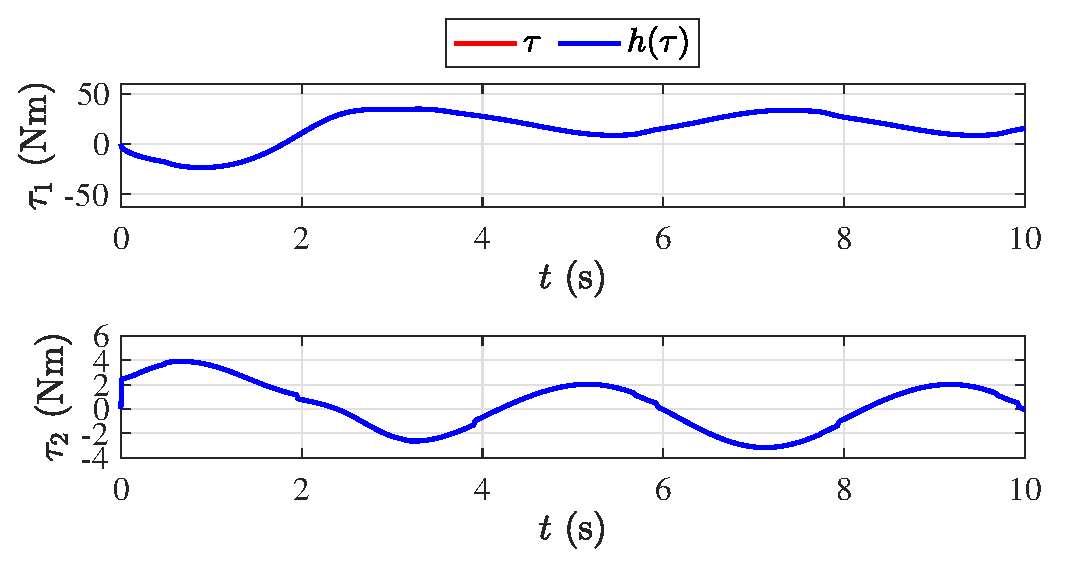
\includegraphics[width=0.4\textwidth]{../fig/fig5.eps}
    \caption{Architecture of the constrained optimization-based neuro-adaptive controller (CONAC).}
  \end{figure}

\end{frame} 


\begin{frame}{Effectiveness of Neuro–Adaptive Control}
  
  
\end{frame}

\subsection{Limitations of Neuro–Adaptive Control}

\begin{frame}{Inherent Challenges in Neuro–Adaptive Control}
  
  Flux theme comes with three pre-defined block style collections.\\
  % Native style (default) available as \verb+\setblockstyle{native}+\\[0.5cm]
  
  \centering
	\begin{minipage}[b]{0.5\textwidth}

	  \begin{block}{Default}
        Block content.
      \end{block}

      \begin{alertblock}{Alert}
        Block content.
      \end{alertblock}

      \begin{exampleblock}{Example}
        Block content.
      \end{exampleblock}      
      
	\end{minipage}
\end{frame}

\begin{frame}{Literature Review}
  
\end{frame}

\subsection{Research Objectives}

\begin{frame}{Research Objectives}
  
\end{frame}

\section{Proposed Method}

\subsection{Constrained Optimization Problem Formulation}

\begin{frame}{Original Problem Formulation}
  \large\textbf{Objectives}:
  \begin{itemize}
    \item Minimize the tracking error by adapting the NN weights $\estwth$.
    \item Guarantee the stability of the system and the NN weights $\estwth$.
  \end{itemize}
  
  \begin{figure}
    \includegraphics[width=0.5\textwidth]{figures/problem.drawio.pdf}
    \caption{Architecture of the constrained optimization-based neuro-adaptive controller (CONAC).}
  \end{figure}

  \small{
    \textit{Notations}: 
    $\mm{M}$: Inertia matrix, $\mm{C}$: Coriolis matrix, $\mm{G}$: Gravity vector, $\mv{\tau}$: Control input, $\mv{q}$: Joint position, $\estwth$: Estimated NN weights.
  }

\end{frame}

\subsection{Adaptation Law Derivation}

\subsection{Stability Analysis}

\section{Numerical Validation}

\subsection{Simulation Setup}
\begin{frame}{2-Link Robotic Manipulator}
    
\end{frame}

\subsection{Simulation Results}

\begin{frame}{Flux}{plots}
	\begin{minipage}{0.56\textwidth}
		\begin{figure}
			\includegraphics[width=\textwidth]{assets/plot.png}
		\end{figure}
	\end{minipage}
	\hfill
	\begin{minipage}{0.38\textwidth}
		\begin{block}{Binary Softmax classifier}
			\centering
			$\sigma(\sum_i w_ix_i + b)$
		\end{block}
		\begin{exampleblock}{Loss function}
			\centering\vspace*{0.1cm}
			$L_i = -log(\frac{e^{f_{y_i}}}{\sum_j e^{f_j}})$\\[0.1cm]
			cross entropy
		\end{exampleblock}
	\end{minipage}
\end{frame}

\begin{frame}{Flux}{tables}
    \begin{table}
      \caption{Largest cities in the world (source: Wikipedia)}
      \begin{tabular}{@{} lr @{}}
        \toprule
        City & Population\\
        \midrule
        Mexico City & 20,116,842\\
        Shanghai & 19,210,000\\
        Peking & 15,796,450\\
        Istanbul & 14,160,467\\
        \bottomrule
      \end{tabular}
      \hspace*{1cm}
          \setlength\extrarowheight{3pt}
      \begin{tabular}{|lr|}
        \hline
        \rowcolor{primaryLight}\color{background}City & \color{background}Population\\
        \hline
        Mexico City & 20,116,842\\
        Shanghai & 19,210,000\\
        Peking & 15,796,450\\
        Istanbul & 14,160,467\\
        \hline
      \end{tabular}
  \end{table}
\end{frame}

\begin{frame}{Weight Norm Constraint}
  \begin{columns}[T,onlytextwidth]
    \column{0.33\textwidth}
      \textbf{Items}
      \begin{itemize}
        \item Cats \item Dogs \item Birds
      \end{itemize}

    \column{0.33\textwidth}
      \textbf{Enumerations}
      \begin{enumerate}
        \item First \item Second \item Last
      \end{enumerate}

    \column{0.33\textwidth}
      \textbf{Descriptions}
      \begin{description}
        \item[Apples] Yes \item[Oranges] No \item[Grappes] No
      \end{description}
  \end{columns}
  \let\thefootnote\relax\footnote{Note the following demo slides are directly taken from metropolis theme. Copyright 2014 Matthias Vogelgesang.\\
Give a look at https://github.com/matze/mtheme/tree/master/demo}
\end{frame}

\section{Conclusion}

\subsection{Conclusion and Future Work}

\begin{frame}{Conclusion}
    
\end{frame}

\section{}
\begin{frame}{}
    \centering \Large
    \emph{Thank you for your attention!}
\end{frame}

\begin{frame}[allowframebreaks]{References}

  \bibliography{../template/refs}
  \bibliographystyle{ieeetr}

\end{frame}

\end{document}